\label{sec:model}


Here we describe the \eapABAC{} family of models  along with formal definitions. \eapABAC{} uses one user-attribute named $\uLabel$ and one object-attribute named $\oLabel$. We define these attributes with predefined semantics. While attributes in general have open-ended semantics, labels ($\uLabel$ and $\oLabel$) are associated with specific semantics. For example, in general, attributes can be set-valued (e.g. roles or clearance) or atomic valued (e.g. age). An attribute value (eg. role, clearance) can be assigned by administrators, self-asserted (e.g. date of birth), or derived from other attributes (e.g. age can be derived from date of birth). Moreover, value of attributes can be ordered or unordered.  On the other hand, labels are set-valued, values are partially ordered and are assigned by administrators. 



We specify \eapABAC{} as a family of models. The basic EAP model (\clabac) presents the minimum elements to define an EAP model. Additionally, we add hierarchies and constraints in \hlabac{} and  \consLabac{} respectively.  \labacOneOneOne{} combines both the hierarchical and constrained models. The components of the \eapABAC{} models are shown in Figure \ref{fig:labac} and the family of the models is schematically presented in Figure \ref{fig:labac-family}.
	% Please add the following required packages to your document preamble:
% \usepackage{booktabs}
\begin{table}
	\centering
	\caption{ \clabac{} Model} %\vspace*{3pt}
	\label{tab:labac-definition}
		\begin{tabular}{|l|}						
		\hline					
				\multicolumn{1}{|c|}{\underline{\textit{I. Sets and relations }}}\\			
				- $U, O$ and $S$ (set of users, objects and sessions resp.)  \\
				- $UL$, $OL$ and $A$ (finite set of user-label values, \\ \hfill object-label values and action resp.) \\
				- $uLabel$ and $oLabel$ (label functions on users and \\ \hfill objects).  $\uLabel: U \to 2^{\UL}$;   $\oLabel: O \to 2^{\OL}$ \\			
				- $\creator: S \to U$, many-to-one mapping from $S$  to $U$ \\
				- $\sessionLabels: S \to 2^{UL}$, mapping from $S$   to    $uLabel$  values. \\ \hfill
				$\sessionLabels(s) \subseteq   uLabel(\creator(s)) $ 	\\ 
				$\langle$ see Section \ref{sec:session-management} for session management functions $\rangle$\\
			%	\hfil [session management functions] \\ 
				\\ \multicolumn{1}{|c|}{\underline{\textit{II. Policy components}}} \\	
				-  $\Policy_a \subseteq \ULV \times  \OLV$,  for action $a \in A$. \\
				- $\Policy = \{ \Policy_a | a \in A  \}$ \\ \\			
				
				\multicolumn{1}{|c|}{\underline{\textit{III. Authorization function}}} \\						
				- \request(s:S,\amem:A,\objmem:O) =	 
					$\exists ul \in \sessionLabels(s) ,$ \\ \hfill $ \exists ol \in oLabel(o)$  $[ (ul,ol) \in$ $\textit{\policy}_a ]  $  		
			
 \\ \hline	
	\end{tabular}
	
\end{table}

%mod


	
\subsection{Basic \eapABAC{} Model}
The elements represented by solid bold lines in Figure \ref{fig:labac} represent the Basic \eapABAC{} Model (\clabac{}). In this model, a set of users, objects and actions (finite set) are represented by $U, O$ and $A$ respectively. Users are associated with a label function named $\uLabel$ and objects are associated with another label function, $\oLabel$. The function $\uLabel$ maps a user to one or more values from the finite set  $UL$ (represented by the double headed arrow from users to UL) and similarly $\oLabel$ maps one object to one or more values from the finite set $OL$ (represented by the double headed arrow from objects to OL). The double headed arrow from $UL$  to users and $OL$ to objects indicate that one user-label value can be associated with more than one user and one object-label value can be associated with more than one object. 

		
 	\begin{figure}
 		\centering
 		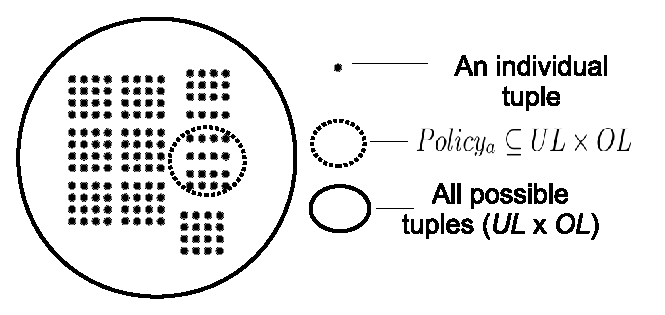
\includegraphics[width=.4\textwidth]{ABAC16/tuples-vs-policy}
 		\caption{Combining subset of tuples in a policy}
 		\label{fig:policy-vs-tuples}
 	\end{figure}	


	
Sessions are denoted by the set $S$. There is a one-to-many mapping from users to sessions. While a user  may have many $\uLabel$ values assigned to him, he can choose to activate any subset of the assigned values in a session. The relation (and function) $\creator$ and $\sessionLabels$ maintain mapping from sessions to users and sessions to $\uLabel$ values respectively.  The $\creator$ and $\sessionLabels$ functions are formally defined in Segment I of Table \ref{tab:labac-definition}. 



In \eapABAC{}, for each action, $a \in A$ we define only one policy, denoted $Policy_a$. A policy is comprised of a subset of tuples from the set of all tuples $UL\times OL$. Relationship between a policy and tuples is schematically shown  in Figure \ref{fig:policy-vs-tuples}. In defining policies, a policy may contain many tuples and a tuple $(ul,ol) \in UL\times OL$ can be used in more than one policy. Thus, a many-to-many relation exists between policies and tuples. Finally, the set \textit{\Policy} contains all individual policies for each action $a \in A$. The formal definition of \textit{\Policy{}} is shown in Segment II of Table \ref{tab:labac-definition}.

The authorization function $\request(s, a, o)$ allows  an access request by a  subject $s \in S$ to perform an action $a \in A$ on an object $o \in O$ if all the following conditions are satisfied - $s$ is assigned a value $ul$;  $o$ is assigned a value $ol$ and the policy for action $a$ contains the tuple $(ul,ol)$. The formal definition of the authorization function is given in Segment III of Table \ref{tab:labac-definition}.


	
		
 	\begin{figure}
 		\centering
 		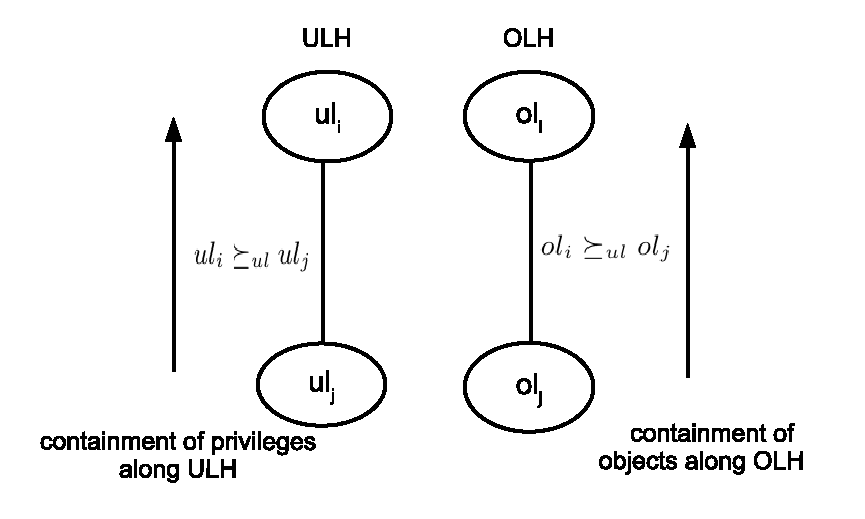
\includegraphics[width=.8\textwidth]{ABAC16/direction-of-implication}
 		\caption{ULH and OLH}
 		\label{fig:direction-of-implication}
 	\end{figure}

		
	
	
	\subsection{Hierarchical \eapABAC{}}
	Hierarchical \eapABAC{} model (\hlabac ) introduces user-label hierarchy ($ULH$) and object-label hierarchy ($OLH$) in addition to the components of \clabac{}. Some elements in \clabac{} are modified in \hlabac{}. The additions and modifications in \hlabac{} from \clabac{} are shown in Table \ref{tab:labach-definition}.
	
	Hierarchy is a convenient way of ranking users and objects. \eapABAC{} achieves ranking on users through $ULH$ and ranking on objects through $OLH$. For two user-label values, $ul_i$ and $ul_j$, when we say $ul_i$ is senior to $ul_j$ (written as $ul_i \udominate ul_j$), we mean that users assigned to $\uLabel$ value $ul_i$  can also exercise all privileges of users who are assigned to value $ul_j$. Similarly, for two object-label values, $ol_i$ and $ol_j$, when we say $ol_i$ is senior to $ol_j$ (written as $ol_i \odominate ol_j$), we mean that objects assigned to value $ol_j$ are also considered as inherited objects for value $ol_i$ for the purpose of authorization. The direction for the containment of privileges and objects along the hierarchy of $ULH$ and $OLH$ is shown in Figure \ref{fig:direction-of-implication}. For containment of objects, in Figure \ref{fig:implied-policy} objects that are assigned value `public', are also considered to be objects that are assigned  value `protected'.
	
	% For example, in Figure \ref{fig:implied-policy}, $protected \odominate public$ and   $ULH$ and $OLH$ is explained in Figure \ref{fig:direction-of-implication}.
	
	When we assign a tuple $(ul_m,ol_n)$ in a policy $\Policy_a$, additional tuples are also implied for $\Policy_a$ because of user-label and object-label value hierarchy. We identify these implied tuples with the notion of a new set $\impliedPolicy$. The implied policy  $\impliedPolicy_a$ includes all tuples of $\Policy_a$ and extra tuples that are implied by every tuples of $\Policy_a$. 
	
	%There is a one-to-one mapping between policies and implied policies.
	

	
		
		% Please add the following required packages to your document preamble:
% \usepackage{booktabs}
\begin{table}
	\centering
	 \captionsetup{justification=centering}
	 \caption{\hlabac{} Model \newline (Additions and modifications to \clabac{})}
	%\caption{  } %\vspace*{3pt}
	\label{tab:labach-definition}
		\begin{tabular}{|l|}						
		\hline								
			\multicolumn{1}{|c|}{\underline{\textit{I. Sets and relations}}} \\		
			%\multicolumn{1}{|c|}{\underline{\textit{(in addition to the basic model)}}} \\		
				  - $\ULH \subseteq \ULV \times \ULV$, partial order ($\succeq_{ul}$) on $UL$  \\
					
	              - $\OLH \subseteq \OLV \times \OLV$, partial order ($\succeq_{ol}$) on $OL$  \\ 
				  - $\sessionLabels(s) \subseteq   \{ ul' | ul \in uLabel(\creator(s)) \land ul \udominate ul' \}$		\\   \\						  				 			 	
		
			\multicolumn{1}{|c|}{\underline{\textit{II. Implied policy}}} \\
				- $\impliedPolicy_a = \{ (\ulvmem_i, \olvmem_j) |  \exists (\ulvmem_m, \olvmem_n) \in \policy_a$[  $ \ulvmem_i \udominate \ulvmem_m \land \olvmem_n \odominate \olvmem_j] \}$	\\ \hfil (explained in Figure \ref{fig:implied-policy})	\\ \\
				
				%- $\textit{\effectivePolicy}_a$ $ = \policy_a \cup \impliedPolicy_a$ \\\\
					
		 	\multicolumn{1}{|c|}{\underline{\textit{III. Authorization function}}} \\
				 
				 	- \request(s:S,\amem:A,\objmem:O) =	 
				 	$\exists ul \in \sessionLabels(s) ,$ \\ \hfill $ol \in oLabel(o)$  $[ (ul,ol) \in$ $\textit{\impliedPolicy}_a ]  $ \\					 
 \hline	
	\end{tabular}
	
\end{table}

%mod



	
 	\begin{figure}[h]
 		\centering
 		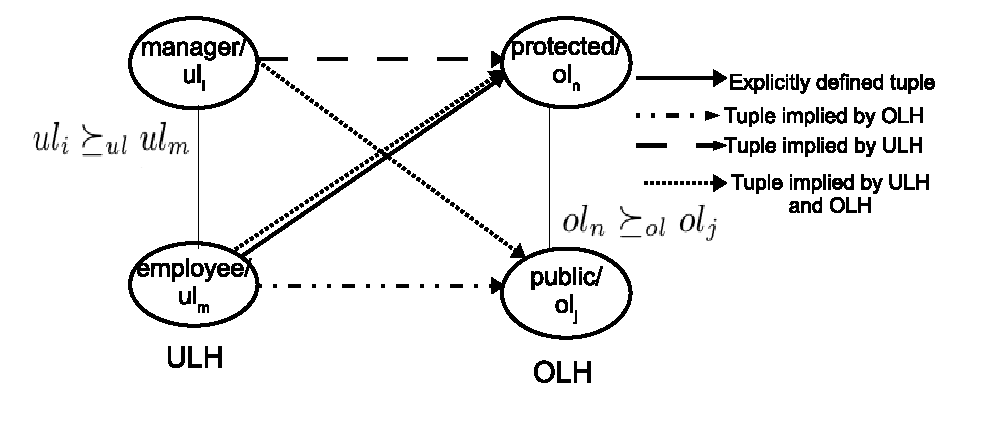
\includegraphics[width=1\textwidth]{ABAC16/implied-policy}
 		\caption{Policy and implied policy}
 		\label{fig:implied-policy}
 	\end{figure}
	
	Implied policy is  explained in Figure \ref{fig:implied-policy}.  For a policy, $\Policy_a = \{(employee, protected)\}$, corresponding implied policy is $\impliedPolicy_a=\{(manager, protected),$ \\$ (manager, public), (employee, protected), (employee, public)\}$. Figure \ref{fig:implied-policy}, further classifies tuples into tuples implied by $ULH$, or $OLH$ or both. Note that authorization function and session function are also modified in Table \ref{tab:labach-definition} to accommodate $ULH$ and $OLH$.
	


	
	
	
	%
 	\begin{figure} 
 		\centering
 		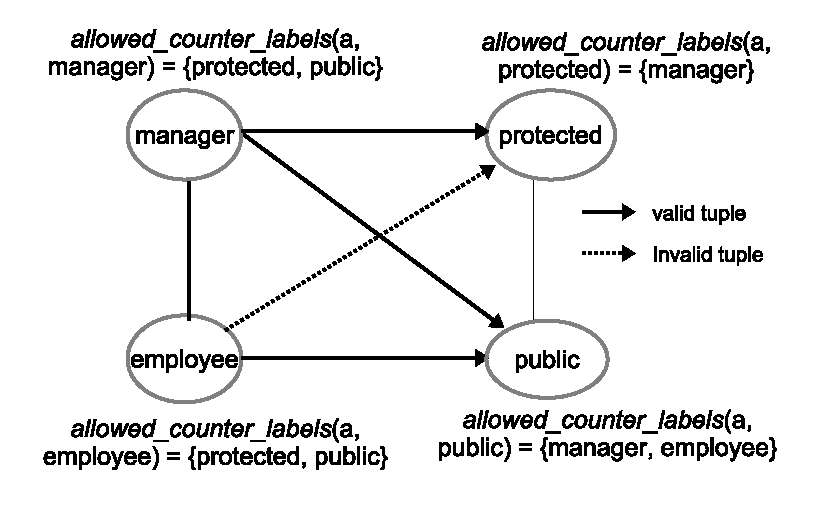
\includegraphics[width=.4\textwidth]{bound-function-explained}
 		\caption{Policy constraints explained with constraint function - \allowedLabels()}
 		\label{fig:bound-function-explained}
 	\end{figure}
	
	\subsection{Constrained \eapABAC{}}
	A general treatment of assignment constraints in ABAC has been covered in  \cite{abcl}. Similarly, role based authorization constraints have been extensively studied in \cite{rcl}.	
	In this section, we specify constraints for the \eapABAC{} model. 
	
	We scope constraints as  means of restricting administrative or user actions. We define two types of constraints - assignment constraints and  policy constraints. Assignment constraints put constraints on user to user-label value assignments,  object to object-label value assignments and session-label value assignments. An example of user-label value assignment constraint is that a user cannot be assigned all of the following values $\{manager, director,$  $employee\}$.  An example of object-label value assignment constraint is that an object cannot be assigned both values - \textit{protected} and \textit{public}. An example of session-label value assignment constraint is that both \textit{manager} and \textit{director} values cannot be activated in the same session.	 Policy constraints, on the other hand,  prevent certain tuples in policies. For example, policy constraints may enforce that an \textit{employee} can never access \textit{protected} objects by restricting the tuple \textit{(employee, protected)}.  
	
	
	\begin{table}
	\centering
	\captionsetup{justification=centering}
	\caption{\consLabac{} Model  (Additions and modifications to \clabac{})} %\vspace*{3pt}
	\label{tab:constraint-definition}
%	\begin{tabular}{|l|l|}
%		\hline
		\begin{tabular}{|l|}						
			\hline					
				
				  \multicolumn{1}{|c|}{\underline{\textit{I. Components added from \clabac{}}}} \\	\\							 
					\textit{{uLabel value assignment constraint}:}\\
						  - CUL = a collection of conflicting user-label values, $\{ CUL_1, CUL_2, ... CUL_n \}$  \\ \hfil  where $CUL_i = \{ ul_1, ... ul_k\}$ \\		\\
						  
 					\textit{{oLabel value assignment constraint:}}\\
						    - COL = a collection of conflicting object-label values,$\{ COL_1, COL_2, ... COL_n \}$  \\ \hfil   where $COL_i = \{ ol_1, ... ol_k\}$ \\ \\
						    
				    \textit{{Session value assignment constraint}:}\\
					    	 - CSL = a collection of conflicting user-label values, $\{ CSL_1, CSL_2, ... CSL_n \}$   \\ \hfil  where $CSL_i = \{ ul_1, ... ul_k\}$ 	\\ \\
								  
					\textit{Policy constraint:}\\ 
						 % - $\allowedLabels(a:A, l:UL/OL) \to 2^{UL/OL}$,  \\ \hfill allowed oLabel values for   given uLabel values \\ \hfill  and vice-versa for action $a$.	\\
						 - \restrictedTuples{} $\subseteq UL \times OL$ \\
						  
			\\ \multicolumn{1}{|c|}{\underline{\textit{II. Derived components}}}	  \\ \\
						  %- $\textit{\policyBound}_a =$ \\ \hfill $ \{ (ul,ol) | \exists ul \in UL \land ol \in \allowedLabels(a,ul)\}  \cap$  \\ \hfill  $\{ (ul,ol) | \exists ol \in OL \land ul \in \allowedLabels(a,ol)\}$  \\    \\				
						  - \policyBound{} = $(UL \times OL) \setminus \restrictedTuples$ \\
			 
			
			\\ \multicolumn{1}{|c|}{\underline{\textit{III. Authorization function}}} \\	\\					
					- \request(s:S,\amem:A,\objmem:O) $\equiv$	 
					$\exists ul \in \sessionLabels(s) ,$ \\ \hfill $ \exists ol \in oLabel(o)$  $[ (ul,ol) \in$ $\textit{\policy}_a \cap \policyBound_a  ]  $  					  
			 
				 	
			 %	\multicolumn{1}{|c|}{\underline{\textit{VI. Sample Enforcement of Assignment Constraints}}} \\
			%		- $ | labels(s) \cap OneElement(CSL) | = 1$, only one  user-label \\ \hfill value can be activated in a session. 
 \\ \hline	
	\end{tabular}
	
\end{table}
	% Please add the following required packages to your document preamble:
% \usepackage{booktabs}
\begin{table}
	\centering
	\caption{ \labac{} Model} %\vspace*{3pt}
	\label{tab:labac-complete-definition}
		\begin{tabular}{|l|}						
		\hline					
				\multicolumn{1}{|c|}{\underline{\textit{I. Basic Components }}}\\			
				- $U, O$ and $S$ (set of users, objects and sessions resp.)  \\
				- $UL$, $OL$ and $A$ (finite set of user-label values, \\ \hfill object-label values and action resp.) \\
				- $uLabel$ and $oLabel$ (label functions on users and  \\ \hfill objects).  $\uLabel: U \to 2^{\UL}$;   $\oLabel: O \to 2^{\OL}$ \\				
				- $\ULH \subseteq \ULV \times \ULV$, partial order ($\succeq_{ul})$ on $UL$  \\	
				- $\OLH \subseteq \OLV \times \OLV$, partial order ($\succeq_{ol}$) on $OL$  \\ 
				- $\creator: S \to U$, mapping from $S$  to $U$ \\
				- $\sessionLabels: S \to 2^{UL}$, mapping from $S$   to $uLabel$  values.\\ \hfill	$\sessionLabels(s) \subseteq   \{ ul' | ul \in uLabel(\creator(s)) \land ul \udominate ul' \}$			\\    			  
			    %- $\allowedLabels(a:A, l:UL/OL) \to 2^{UL/OL}$,  \\ \hfill allowed oLabel values for   given uLabel values \\ \hfill  and vice-versa for action $a$.	\\\\
 			   - $\restrictedTuples \subseteq UL \times OL$ \\
 			   - \textit{CUL, COL, CSL} (conflicting set of $\uLabel, \oLabel$\\ \hfill and session-label values) \\$\langle$ see Section \ref{sec:session-management} for session management functions $\rangle$\\
			    
			   \\	\multicolumn{1}{|c|}{\underline{\textit{II. Policy components}}} \\	
			   	-  $\Policy_a \subseteq \ULV \times  \OLV$,  for action $a \in A$. \\
			   	- $\Policy = \{ \Policy_a | a \in A  \}$ \\ \\
			    
			    \multicolumn{1}{|c|}{\underline{\textit{III. Derived components}}} \\
			    - $\impliedPolicy_a = \{ (\ulvmem_i, \olvmem_j) |  \exists (\ulvmem_m, \olvmem_n) \in \policy_a$[ \\ \hfill $ \ulvmem_i \udominate \ulvmem_m \land \olvmem_n \odominate \olvmem_j] \}$	\\
			     - $\textit{\policyBound} = (UL \times OL) \setminus \restrictedTuples$ \\
			    
			    
				\\ \multicolumn{1}{|c|}{\underline{\textit{IV. Authorization function}}} \\ 						
				- \request(s:S,\amem:A,\objmem:O) =	 
					$\exists ul \in \sessionLabels(s), $ $\exists ol $ \\ \hfill   $ \in oLabel(o) [ (ul,ol) \in$ $\textit{\impliedPolicy}_a \cap  \textit{\policyBound}]  $  		
			
 \\ \hline	
	\end{tabular}
	
\end{table}

%mod


		
		 
		 
	Assignment constraints are specified by defining a set of conflicting $\uLabel$, $\oLabel$ and \textit{session} values denoted by $COL$, $CUL$ and $CSL$ respectively in Table \ref{tab:constraint-definition}.  The constraint that an object cannot be assigned both values - `protected' and `public' is specified as $COL=\{\{public, protected\}\}$ and $ |\oLabel(o) \cap OneElement(COL)| \le 1$ where function $OneElement()$ returns one element from its input set. (we use the same concept of \textit{OneElement()} from \cite{rcl}).  Similarly, other  assignment constraints can also be formulated. Note that user-label value assignment constraints can be used to configure  Static Separation of Duty, while session constraints can be used to enforce some aspects of  Dynamic Separation of Duty \cite{dsod}.


 	\begin{figure}
 		\centering
 		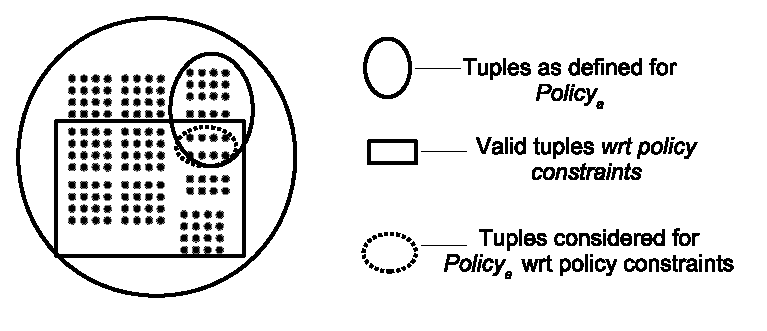
\includegraphics[width=.6\textwidth]{ABAC16/tuples-vs-valid-tuples}
 		\caption{Restricting policies with policy constraints}
 		\label{fig:tuples-vs-valid-tuples}
 	\end{figure}	


	Policy constraints are defined by using \textit{\restrictedTuples}.  For a tuple, $(ul_r,ol_r) \in \restrictedTuples$, if it is included in a policy, $\Policy_a$, it would be ignored in the computation of authorization decision. For convenience we define a derived set \textit{\policyBound} as all possible tuples minus \textit{\restrictedTuples}. \textit{\restrictedTuples} and \textit{\policyBound} are defined in Table \ref{tab:constraint-definition}. Policy constraint is explained schematically in Figure \ref{fig:tuples-vs-valid-tuples}.
	
	In \consLabac{}, we include constraint policies beyond authorization policies. While, authorization policies establish relationship only between user-label and object-label values (along with actions), constraint policies go beyond. For example, constraint policies may consider relationship between \textit{UL} and \textit{OL} (policy constraints), $UL$ and $UL$ (\textit{\uLabel/session} value assignment constraints), $OL$ and $OL$ (\textit{\oLabel} value assignment constraints), \textit{S} and \textit{UL} (cardinality constraints on session value assignments) and so on.  As a result, constraint policies in \consLabac{} include logical formulas as well as enumerated tuples.
	
	
	
	
	\subsection{The Combined Model (\labacOneOneOne{})}
	
	The combined model, \labacOneOneOne{} (shown in Table \ref{tab:labac-complete-definition}), combines elements from both \hlabac{} and \consLabac{} models.  Segment I of Table \ref{tab:labac-complete-definition} presents all basic sets and relations. Policy components and derived components are shown in Segment II and  III respectively. Finally, authorization decision function is defined in Segment IV.
	

